\section{Preliminary investigation}\label{sec:preinvestigation}

\subsection{Medarbejder-mål tabel}\label{mmt}
%text goes here
\begin{center}
\begin{tabular}{ |p{100pt}|p{100pt}|p{100pt}| }
    \hline
    Medarbjeder & Opgave & Mål \\
    \hline\hline
    Sælgere
    & udføre salg & salget er udført \\
    \hline
    & køre forberelse & sælger er klar til at køre \\
    \hline
    Lagermedarbejder
    & påfyld bil & bil er fuld \\
    \hline
    & modtag ny levering & levering er i kølerbokse \\
    \hline
    Depotchef
    & registrer salg of dagsomstætning på biller & aktiviter fra dagen før er bogført \\
    \hline
    & udprinte odrer & orderer er klar til sælgere \\
    \hline
    & lave router & router er klar til sælgerer \\
    \hline
    & bestemmer lager orden & lageret passer markets efterspørgsel \\
    \hline
\end{tabular}
\end{center}

\begin{center}
\begin{tabular}{ |p{90pt}|p{90pt}|p{90pt}|p{90pt}| }
    \hline
    Medarbjeder & Opgave & Mål & Trin i opgave \\
    \hline\hline
    Sælgere
    & udføre salg & salget er udført &
    - test1 \\
    &&&
    - test2 \\
    \hline
    & køre forberelse & sælger er klar til at køre &
    - test1 \\
    &&&
    - test2 \\
    \hline
    Lagermedarbejder
    & påfyld bil & bil er fuld &
    - test1 \\
    &&&
    - test2 \\
    \hline
    & modtag ny levering & levering er i kølerbokse &
    - test1 \\
    &&&
    - test2 \\
    \hline
    Depotchef
    & registrer salg of dagsomstætning på biller & aktiviter fra dagen før er bogført &
    - test1 \\
    &&&
    - test2 \\
    \hline
    & udprinte odrer & orderer er klar til sælgere &
    - test1 \\
    &&&
    - test2 \\
    \hline
    & lave router & router er klar til sælgerer &
    - test1 \\
    &&&
    - test2 \\
    \hline
    & bestemmer lager orden & lageret passer markets efterspørgsel &
    - test1 \\
    &&&
    - test2 \\
    \hline
\end{tabular}
\end{center}

\subsection{Mock ups og designprincipper}
Når det kommer til at designe en brugergrænseflade til sit system, er der indtil flere overvejelser man skal igennem. Målet er at gøre brugergrænsefladen så brugervenlig, hurtig og intuitiv som mulig. Dette afsnit vil derfor gennemgå hvilke overvejelser der er indgået i beslutningen for designet af de anvendte mock ups.

\subsubsection{Farver}
Farver i et professionelt UI system kan være en definerende faktor. Farven må ikke være for meget til stede, men giver blot en identitet til programmet. I programmer som Spotify og Visual Studio Code har de begge en identitetsfarve, henholdsvis grøn og blå, men farven ses kun vigtige steder i programmet. 
\begin{figure}
    \centering
    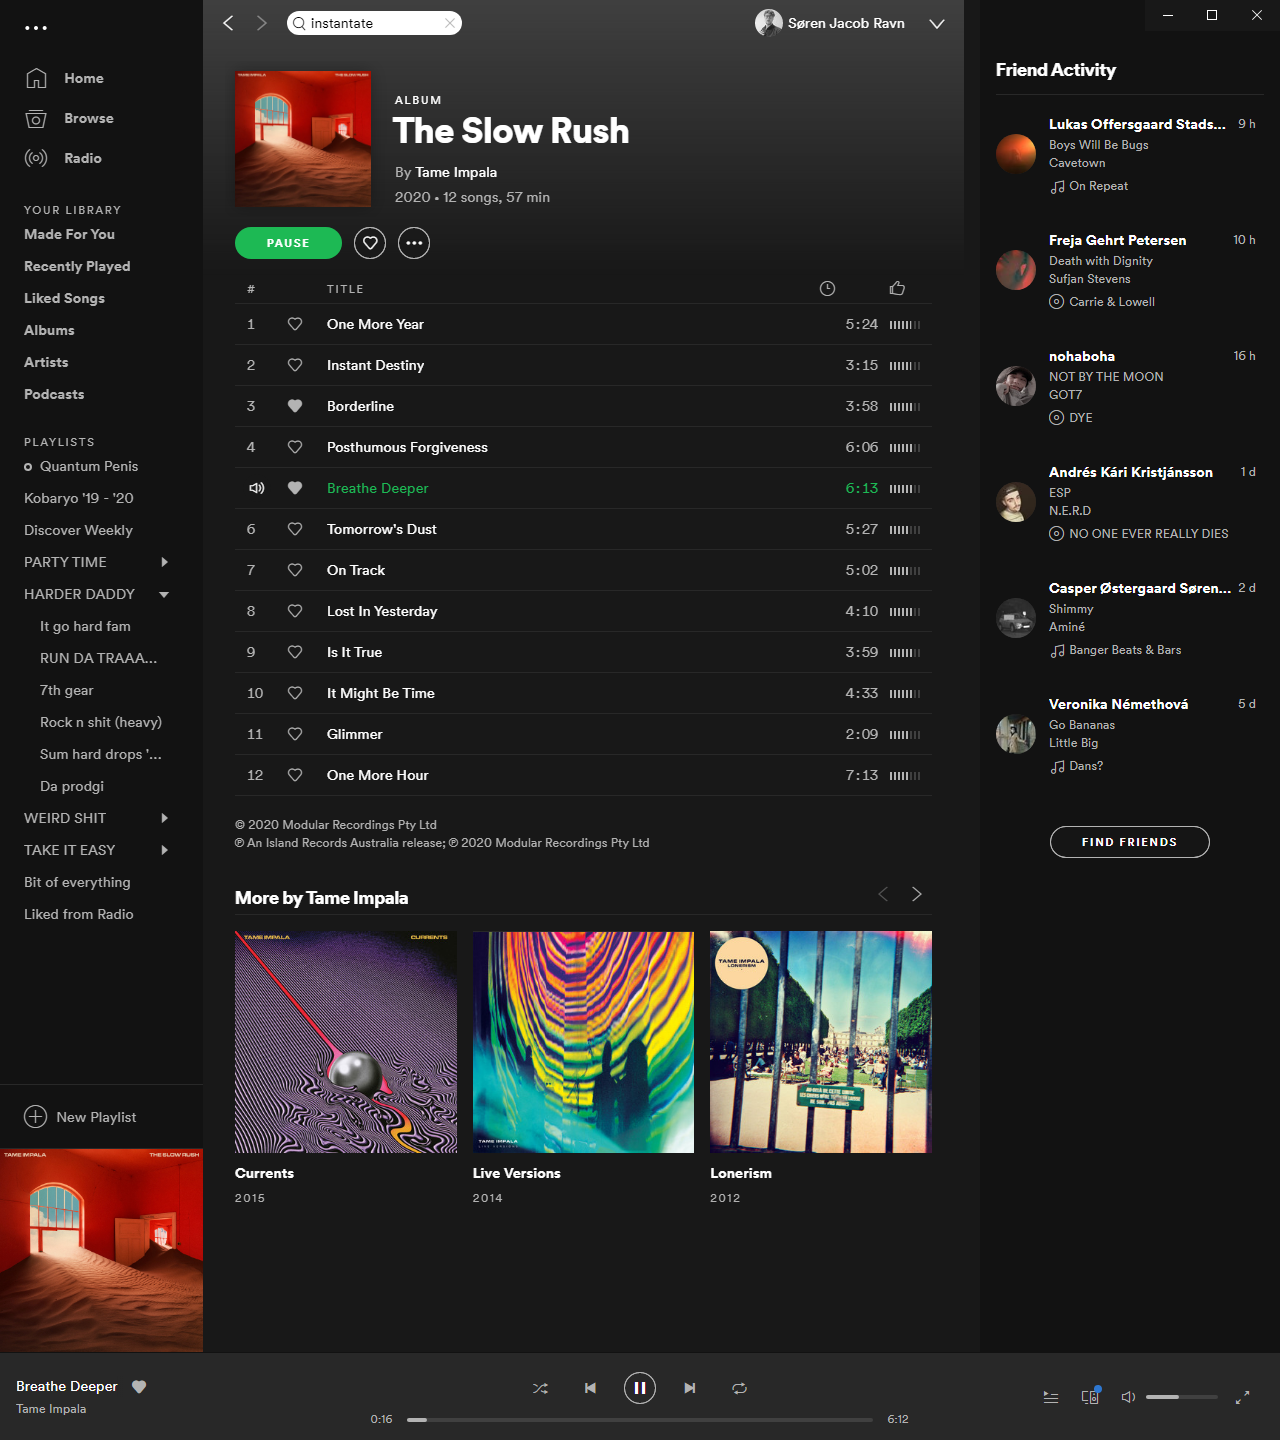
\includegraphics[width=\textwidth]{figures/Preliminary/Spotify.png}
    \label{fig:spotify}
\end{figure}